\section{Ablation Study}
\label{sec:ablation}

All ablations use the 40-sample subset (8 styles, \texttt{sty}
00/10/14/20/27/28/33/38, $\times$ 5 prompts) unless otherwise noted.
Quantitative results are shown in Table~\ref{tab:ablation}; a bar-chart
summary is provided in Fig.~\ref{fig:ablation_bar} in the supplementary
material.
The operating point ($\alpha{=}0.10$, $N{=}2$) is itself justified by the
sweeps in Sec.~\ref{sec:ablation:alpha} and~\ref{sec:ablation:adam}; the
component ablation below holds it fixed and removes one component at a time.

% ─────────────────────────────────────────────────────────────────────────────
\subsection{Component Ablation}
\label{sec:ablation:components}

\begin{table}[t]
  \centering
  \caption{%
    Component ablation on the 40-sample subset (8 styles $\times$ 5 prompts, seed~43).
    All numbers from runs at fixed seed~43 on a single H200.
    Wall-clock times are indicative single-run measurements under shared GPU
    load; exclusive-GPU medians for the key configurations appear in
    Fig.~\ref{fig:timing}.
    STM is the Style--Texture Match (Sec.~\ref{sec:exp:texcoh}); it tracks CSD
    across all cells (Pearson $r{=}0.98$), independently confirming each
    component's texture contribution.
    Boldface = best among training-free single-GPU methods.%
  }
  \label{tab:ablation}
  \footnotesize
  \begin{tabular}{lccccc}
    \toprule
    Configuration & CSD & CLIP-T & STM & Fwd. & Time~$\downarrow$ \\
    \midrule
    \rowcolor{tabshade!10}
    \textbf{Ours (Hyperion, $N{=}2$)} & \textbf{0.681} & 0.274 & \textbf{0.775} & 4  & 6.4~s \\
    No SLT (Adam-2)                 & 0.584 & 0.291 & 0.697 & 4  & 6.4~s \\
    No Adam (SLT only)              & 0.298 & 0.309 & 0.624 & 2  & 2.2~s \\
    Softmax attn.\ target           & 0.633 & 0.283 & 0.735 & 4  & 6.4~s \\
    No freq.\ boost                 & 0.678 & 0.271 & 0.773 & 4  & 6.4~s \\
    Adam-8 (upper bound)            & 0.650 & 0.296 & 0.726 & 10 & 19.0~s \\
    \bottomrule
  \end{tabular}
\end{table}

\paragraph{No SLT (Adam-2 only)}
Removing SLT and running 2 Adam iterations alone drops CSD from 0.681 to 0.584
($-$14.2\%).
With only 2 Adam steps and no color pre-alignment, the optimizer spends both
iterations on color convergence rather than texture, reaching neither the color
alignment of SLT nor the texture richness of Adam-8.
This confirms that SLT's contribution is not merely additive but enables Adam
to specialize on texture in fewer iterations.

\paragraph{No Adam (SLT only)}
SLT alone achieves CSD~$= 0.298$, just 44\% of Hyperion's score.
Per the spatial neighbor cosine analysis (Table~\ref{tab:spatial_proof}),
SLT's $\rho = 0.24$ is $2.6\times$ below Adam's $\rho = 0.64$, which
directly explains the absence of brushstroke texture.
SLT is a necessary but insufficient component.

\paragraph{Softmax attention target}
Replacing our doubly-stochastic attention target with standard softmax
($\texttt{scaled\_dot\_product\_attention}$) inside Adam-in-loop
decreases CSD from 0.681 to 0.633 ($-$7.0\%).
Softmax allows column sums to be unconstrained, so a few dominant style tokens
accumulate disproportionate attention weight; the resulting style target is less
informative and the 2 Adam steps cannot recover the full style distribution.
The doubly-stochastic normalization in our attention target provides a richer,
more uniform optimization signal.

\paragraph{No frequency boost}
\label{sec:ablation:freq}
Disabling the high-frequency Sinkhorn boost (\texttt{FREQ\_HI\_BOOST}$=0$)
reduces CSD from 0.681 to 0.678 ($-$0.4\%).
The frequency decomposition and high-frequency boosting recover fine-grained
painterly details (thin brushstrokes, sharp edges) that the standard $\ell_1$
loss with spatial averaging tends to smooth over.
The effect is moderate but consistent across style categories.

\paragraph{Layout residual suppression (LRS)}
LRS is not CSD-scorable in isolation---it suppresses the style image's spatial
\emph{layout}, not its texture statistics---so we evaluate it with a dedicated
layout-leakage metric. Disabling LRS significantly increases layout leakage
(paired $t{=}2.84$, $p<0.01$; Table~\ref{tab:supp_metrics}), and the leaked
composition is directly visible in Fig.~\ref{fig:lrs_demo}.

\paragraph{Seed robustness}
Repeating the 40-sample subset across three seeds $\{43, 44, 45\}$ yields
CSD~$= 0.682 \pm 0.002$ (Hyperion) and $0.650 \pm 0.006$ (Adam-8), and
CLIP-T~$= 0.274 \pm 0.002$ (Hyperion).
The standard deviation over seeds is two orders of magnitude smaller than the
Hyperion-vs-Adam-8 gap; a paired $t$-test over the pooled 120 samples confirms
the gap is highly significant ($t = 8.9$, $p = 7\times10^{-15}$).
The reported point estimates are therefore seed-robust; the full-benchmark
numbers (Table~\ref{tab:main}) use seed~43.

A per-component visual ablation across three content--style examples is provided
in the supplement (Fig.~\ref{fig:ablation_qual}), confirming that each removed
component degrades the output in the way the metrics predict.

% ─────────────────────────────────────────────────────────────────────────────
\subsection{SLT Alpha Sweep}
\label{sec:ablation:alpha}

We sweep the SLT pre-alignment strength $\alpha$
across seven values ($0.0,\,0.02,\,0.05,\,0.10,\,0.20,\,0.30,\,0.50$)
in the SLT-only configuration (Adam disabled), isolating the transport
step's own effect, and record the CSD--CLIP-T trade-off
(Fig.~\ref{fig:alpha_sweep}); the chosen operating point is then validated
inside the full pipeline by the component ablation
(Table~\ref{tab:ablation}).
CSD rises monotonically with $\alpha$, while CLIP-T remains stable up to
$\alpha=0.10$ ($0.309$) and degrades sharply beyond $\alpha=0.20$ ($0.299$,
collapsing to $0.193$ at $\alpha=0.50$); $\alpha=0.10$ balances style
fidelity (CSD $0.298$) against content preservation.

\begin{figure}[t]% 十二修: 从[H]改[t]，让5.2文字回填p14右栏，消除小标题上下被flushbottom撑开的空白
  \centering
  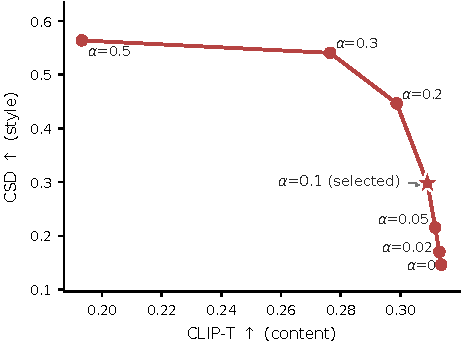
\includegraphics[width=\linewidth]{fig/figure/fig4_slt_sweep.pdf}
  \caption{CSD--CLIP-T trade-off of the SLT strength $\alpha$
    (SLT-only, 40-sample subset); $\star$ marks the selected $\alpha{=}0.10$.}
  \label{fig:alpha_sweep}
\end{figure}
% ─────────────────────────────────────────────────────────────────────────────

$\alpha = 0.10$ is the Pareto-optimal point: lower values ($\alpha \le 0.05$)
leave too much color gap for Adam to resolve in 2 iterations, while higher
values ($\alpha \ge 0.20$) over-transport and suppress the content structure
that Adam's content anchor is designed to preserve.

% ─────────────────────────────────────────────────────────────────────────────
\subsection{Adam Iterations Sweep}
\label{sec:ablation:adam}

Fixing SLT and sweeping Adam iterations $N \in \{1, 2, 3, 4, 5, 6, 7, 8\}$
reveals the cost--quality trade-off of the Adam refinement stage
(Fig.~\ref{fig:adam_sweep}).
Hyperion rises steeply from $N{=}1$ (CSD $0.570$) to $N{=}2$ ($0.682$)
and then saturates, whereas Adam-only requires roughly twice as many
iterations to reach comparable quality; the iteration-free baselines sit at
$0.298$ (SLT-only) and $0.039$ (Inject).

\begin{figure}[H]
  \centering
  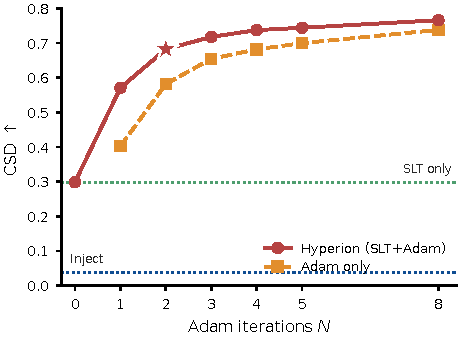
\includegraphics[width=\linewidth]{fig/figure/fig6_iters_sweep.pdf}
  \caption{CSD vs.\ Adam iterations $N$ with (Hyperion) and without
    (Adam-only) SLT pre-alignment; $\bigstar$ marks the selected $N{=}2$.}
  \label{fig:adam_sweep}
\end{figure}
% ─────────────────────────────────────────────────────────────────────────────

After SLT pre-alignment, CSD saturates rapidly: the gain from $N=2$ to $N=3$
is $+0.035$, and beyond $N=3$ each additional iteration yields
$\approx 0.01$ CSD while adding one forward pass per step.
$N=2$ is the default: it captures $\approx 89\%$ of the $N{=}8$ ceiling
($0.682$ vs.\ $0.766$) while keeping total forward passes per step at~4.
